%\newpage
%\subsection{Dataset}

\subsubsection{MEG preprocessing}

One hundred and two subjects performed a similar reading task to the one
described above in the MEG scanner. The raw MEG data was bandpass-filtered between 0.1 and 40Hz using MNE-Python
default parameters \citep{gramfort2013meg, gramfort2014mne}. Specifically, we
used a zero-phase finite impulse
response filter (FIR) with a Hamming window and with transition bands of 0.1Hz
and 10Hz for the low and high cut-off frequencies. The raw data was then
segmented 100ms before word onset and 1s after
word onset ($t=0$ms corresponds to word onset). Finally, each resulting
segment was baseline-corrected between -100ms and 0ms, and decimated by 5 and
thus led a sampling frequency of 240Hz. The average responses across words is
displayed in Fig.~\ref{fig:meg_evoked}.
For each subject and each time sample relative to word onset, we
build an observation matrix $Y \in \mathbb{R}^{m \times d_y}$ of $m\approx$ 2,700 words
by $d_y=301$ MEG channels (273 magnetometers and 28 compensation channels). Each
of the columns of $Y$ is normalized to have zero mean and unit variance.

We use the same features as for the fMRI experiments, except that the features
were not convolved by an hemodynamic response function. This yields an $X \in \mathbb{R}^{m \times d_x}$
matrix of $m\approx$ 2,700 words by $d_x=4$ features for each subject. Each of
the columns of $X$ is normalized to have a mean and a standard deviation of 0
and 1 respectively.

We compare B2B against other methods following the same procedure as for the
fMRI experiments, except that the searchlight swipes across time samples, and
is trained across all MEG channels.


\begin{figure}[t!]
  \begin{minipage}[c]{0.6\textwidth}
    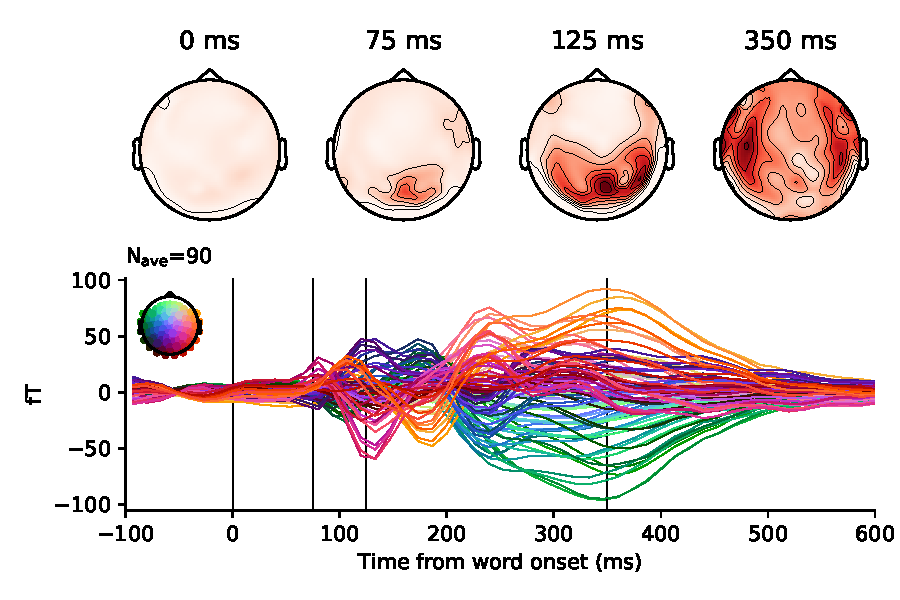
\includegraphics[width=\textwidth, trim=0cm 0cm 0cm 0cm, clip=True]{figures/meg_evoked.pdf}
  \end{minipage}\hfill
  \begin{minipage}[c]{0.4\textwidth}
    \caption{A hundred subjects read approximately 2,700 words while their
    brain activity was recorded with MEG. Top. Average brain response to words
    (word onset at t=0 ms), as viewed from above the head (red= higher gradient
    of magnetic flux). Bottom. Each line represents a magnetometer, color-coded
    by its spatial position. Posterior responses, typical of primary visual
    cortex activity, peak around 100 ms after word onset and are followed by
    an anterior propagation of activity typical of semantic processing in the
    associative cortices.
    }
    \label{fig:meg_evoked}
  \end{minipage}
\end{figure}


\begin{figure}
  %\vspace{-12ex}
  \begin{center}
    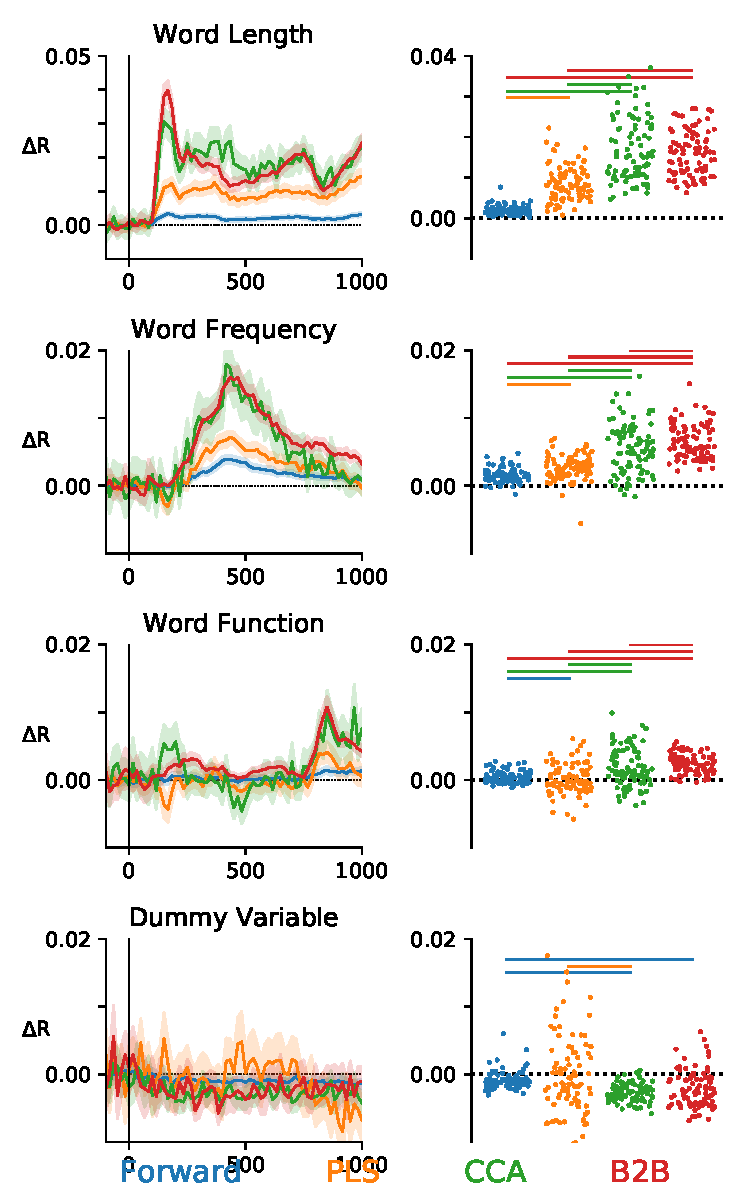
\includegraphics[width=0.6\textwidth,
                     trim=0cm 0cm 0cm 0cm, clip=True]{figures/meg.pdf}
  \end{center}
  %\vspace{-5ex}
  \caption{Multiple models (color-coded) are compared on their ability to
  reliably predict single-trial MEG signals evoked by words. Left. Average
  improvement of correlation coefficient $\Delta R$ for each of the four
  features (rows). Error bars indicate standard error of the mean (SEM) across
  subjects. Right. Average $\Delta R$ across time for each subject (dots). Top
  horizontal lines indicate when B2B significantly outperforms other methods
  (red) and vice versa. \label{fig:meg_results}
}
\end{figure}


\subsubsection{Results}
We compared the ability of Forward regression, Backward regression, CCA, PLS and
B2B to estimate the causal contribution of four distinct but linearly-correlated features
on brain evoked responses to words.

As expected, the Backward model reveals a similar decoding time course for Word
Length and Word Frequency, even though these features are known to specifically
influence early and late MEG responses respectively \citep{kutas2011thirty}. In
addition, the same decoding time course was observed for the dummy variable.
Once again, these results illustrate that Backward modeling cannot be used to estimate the
causal contribution of correlated features.

We thus focus on the four remaining methods (i.e. Forward Regression, PLS, CCA,
and B2B) and estimate their $\Delta R$ (i.e. the improvement of Y prediction
induced by the introduction of a given feature into the model,as described in
Algorithm \ref{algorithm:b2b_fi}). Contrary to the Backward Model, none of the
models predicted the Dummy Variable to improve the $Y$ prediction: all $\Delta R
< 0$ (all $p > .089$).

Figure~\ref{fig:meg_results} shows, for each model, the effects obtained across
time (left) and subjects (right).

Word Length and Word Frequency improved the prediction performance of all
methods: $\Delta R>0$ for all models (all $p<0.0001$). As expected, the time
course associated with Word Length and Word Frequency rose from $\approx$ 100 ms
and from $\approx$ 400 ms respectively. Furthermore, Word Function improved the
prediction performance of all models (all $p < 0.0002$) except for
PLS~($p=0.7989$). Overall, these results confirm that Word Length, Word
Frequency and Word Function specifically improve the prediction of specific periods of brain
responses to words, and thus form plausible independent causal contributors.

We compare B2B to other models across subjects (Fig.~\ref{fig:meg_results}
right). For both Word Length and Word Frequency, B2B outperforms all models (all $p < 0.0001$).
For "Word Function", B2B outperforms all models (all $p < 0.0001$) but CCA ($p<0.0001$).
Overall, these results show that B2B generally compares favorably against baseline models.
